\documentclass[11pt,a4paper]{article}

\usepackage{lmodern}
\DeclareMathSizes{10.95}{10}{10}{10}
\DeclareMathSizes{10}{10}{10}{10}
\DeclareMathSizes{9}{10}{10}{10}
\usepackage[margin=0.8in]{geometry}
\usepackage{amsmath,amssymb}
\usepackage{booktabs}
\usepackage{float}
\usepackage{tabularx}
\usepackage{array}
\usepackage{graphicx}
\usepackage{xcolor}
\usepackage{listings}
\usepackage{fancyhdr}
\usepackage{caption}
\usepackage{enumitem}
\usepackage{microtype}
\usepackage{tikz}
\usetikzlibrary{arrows.meta,positioning,shapes.geometric,calc}
\usepackage[hidelinks]{hyperref}

\definecolor{codebg}{RGB}{246,247,249}
\definecolor{codeblue}{RGB}{33,82,145}
\definecolor{codegreen}{RGB}{27,116,70}
\definecolor{codestr}{RGB}{140,40,90}

\lstdefinelanguage{Rust}{
  morekeywords={as,break,const,continue,else,enum,false,fn,for,if,impl,in,let,loop,
    match,mod,move,mut,pub,ref,return,self,Self,static,struct,trait,true,type,use,
    where,while,Some,None,Ok,Err},
  sensitive=true,
  morecomment=[l]{//},
  morestring=[b]",
}

\lstset{
  language=Rust,
  basicstyle=\ttfamily\footnotesize,
  keywordstyle=\color{codeblue}\bfseries,
  commentstyle=\color{codegreen}\itshape,
  stringstyle=\color{codestr},
  backgroundcolor=\color{codebg},
  numbers=left,
  numberstyle=\tiny\color{gray},
  numbersep=6pt,
  frame=single,
  rulecolor=\color{gray!40},
  xleftmargin=1.5em,
  framexleftmargin=1.2em,
  breaklines=true,
  columns=fullflexible,
  keepspaces=true,
  showstringspaces=false,
  captionpos=t,
  aboveskip=6pt,
  belowskip=8pt,
}
\lstdefinestyle{plain}{
  language={},
  numbers=none,
  xleftmargin=0pt,
  framexleftmargin=0pt,
  backgroundcolor=\color{codebg},
  basicstyle=\ttfamily\scriptsize,
}

\pagestyle{fancy}
\fancyhf{}
\fancyhead[L]{\small CSE/PC/B/S/314 Computer Networks Lab --- Group Project}
\fancyhead[R]{\small ARP (UDP) \& Encrypted Telnet (TCP)}
\fancyfoot[C]{\small\thepage}
\renewcommand{\headrulewidth}{0.4pt}

\setlength{\parskip}{4pt}
\setlength{\parindent}{0pt}
\setlist{itemsep=2pt,topsep=3pt,leftmargin=1.5em}
\captionsetup{font=small,labelfont=bf}
\captionsetup[lstlisting]{font=small,labelfont=bf,skip=4pt}

\begin{document}

\begin{center}
  {\Large\bfseries CSE/PC/B/S/314 Computer Networks Lab --- Group Project Report}\\[0.25cm]
  {\large Socket Implementation of ARP (UDP) and Encrypted Telnet via RSH (TCP) in Rust}
\end{center}
\vspace{0.1cm}
\hrule
\vspace{0.25cm}

\tableofcontents
\newpage

% ================================================================ 1
\section{Overview}

\subsection{Project Scope}
The mini group project requires implementing protocols across the Network, Transport, and Application layers using TCP/UDP sockets in standard-library Rust (\texttt{std::net}, zero external crates):
\begin{itemize}
  \item \textbf{ARP (\texttt{arp/}, Basket~1):} Implements the Address Resolution Protocol (RFC~826) over connectionless UDP datagrams (default port \texttt{4000}), enhanced with static-entry spoofing protection, dynamic MAC-change warnings, strict packet/sender validation, self-lookup short-circuiting, bounded UDP retries, and interactive cache flushing.
  \item \textbf{Encrypted Telnet via RSH (\texttt{rsh/}, Basket~3):} Implements an encrypted remote-terminal (Telnet-equivalent) service over TCP (default port \texttt{2222}) instead of plaintext Telnet. Split across four crates---\texttt{rsh-crypto} (64-bit RSA, signatures, and directional stream cipher), \texttt{rsh-main} (\texttt{rsh} server/client), \texttt{rsh-keygen}, and \texttt{rcp}---it streams interactive remote shell I/O and file transfers over an authenticated, encrypted channel.
\end{itemize}

\subsection{ARP Theory (RFC 826) and Hardening}
In IPv4-over-Ethernet networks, 32-bit network-layer IPv4 addresses must be translated into 48-bit link-layer MAC addresses before a frame can be transmitted on a local segment:
\begin{enumerate}
  \item \textbf{Local Cache Lookup:} Before sending any packet on the wire, a host checks its local ARP cache. A valid (unexpired) hit resolves immediately in memory; entries age out after a Time-To-Live (TTL, 60\,s here) so stale hardware mappings do not persist forever.
  \item \textbf{Request and Reply:} On a miss, the requester broadcasts a 28-byte ARP Request (\texttt{OP=1}) containing its Sender Hardware Address (SHA), Sender Protocol Address (SPA), and the Target Protocol Address (TPA), with Target Hardware Address (THA) zeroed. The responder returns an ARP Reply (\texttt{OP=2}) placing the resolved MAC in SHA and swapping the requester's values into THA/TPA.
  \item \textbf{Passive Learning and ARP Spoofing:} Standard RFC~826 is stateless and trusts every incoming \texttt{(SPA, SHA)} pair. While passive learning lets peers discover each other dynamically without static configuration, an attacker can send forged requests claiming the gateway IP (\texttt{192.168.1.1}) with its own MAC (\emph{ARP cache poisoning}). Our modified server defends against this by marking preloaded infrastructure hosts as \texttt{Static} (immutable), rejecting invalid senders (\texttt{0.0.0.0} or zero/multicast MACs), and emitting explicit warnings if a dynamic host changes its MAC.
  \item \textbf{UDP Encapsulation Overlay:} Emitting raw EtherType \texttt{0x0806} frames requires privileged raw-socket access (\texttt{root} / \texttt{CAP\_NET\_RAW}). Carrying the exact 28-byte RFC~826 payload inside UDP datagrams keeps the wire layout authentic while running portably in unprivileged user space.
\end{enumerate}

\subsection{Encrypted Telnet (RSH) Theory}
Classic Telnet (RFC~854) streams interactive terminal keystrokes and shell output in cleartext over TCP, exposing passwords, commands, and host identity to eavesdropping or spoofing. Our Encrypted Telnet (\texttt{rsh}) preserves Telnet's interactive remote-shell model (piping client stdin to a server-side \texttt{sh -i} or \texttt{cmd.exe} process and streaming stdout/stderr back over TCP) while adding three security layers:
\begin{enumerate}
  \item \textbf{Server Identity (TOFU):} The server presents an RSA public host key $(n_h, e)$. The client checks \texttt{known\_hosts} using Trust-On-First-Use: an unseen host is recorded, whereas a changed key aborts the connection to prevent man-in-the-middle interception.
  \item \textbf{Confidentiality via Hybrid Encryption:} The client generates a 32-byte random session key $K$, encrypts it in 7-byte blocks with the server's RSA public key ($c = m^e \bmod n_h$, $e=65537$, $n_h = pq \ge 2^{62}$), and both sides initialize independent \texttt{xoshiro256}-style stream ciphers keyed by $(K, \text{c2s})$ and $(K, \text{s2c})$. Every terminal frame (\texttt{Shell}, \texttt{Data}, \texttt{Exit}) and file transfer (\texttt{rcp}) is encrypted after this point.
  \item \textbf{Client Authentication:} The client proves possession of its private key $d_c$ by signing $\text{``rsh-auth''} \parallel K \parallel \text{user}$ with $s = H(x)^{d_c} \bmod n_c$, where $H$ is an FNV-1a-based 64-bit digest. The server checks \texttt{authorized\_keys} and verifies $s^e \equiv H(x) \pmod{n_c}$.
\end{enumerate}

% ================================================================ 2
\section{Design}

\subsection{Purpose of the Programs}
\begin{itemize}
  \item \textbf{\texttt{arp}:} Demonstrates RFC~826 binary framing over UDP, local TTL caching, bounded client retransmission on packet loss, self-IP resolution, passive dynamic host learning, and static-entry protection against ARP poisoning.
  \item \textbf{Encrypted Telnet (\texttt{rsh}, \texttt{rsh-keygen}, \texttt{rcp}):} Replaces plaintext Telnet with an encrypted remote-terminal channel over length-prefixed TCP frames, 64-bit RSA key exchange (Miller--Rabin primality testing), key-file management, bidirectional shell I/O streaming, and remote file transfer.
\end{itemize}

\subsection{Structure Diagrams}

Figure~\ref{fig:arch} shows the modular organization of both Cargo projects, and Figure~\ref{fig:handshake} illustrates the Encrypted Telnet (\texttt{rsh}) handshake and remote-terminal message exchange.

\begin{figure}[H]
\centering
\begin{minipage}[t]{0.48\textwidth}
\centering
\resizebox{\linewidth}{!}{%
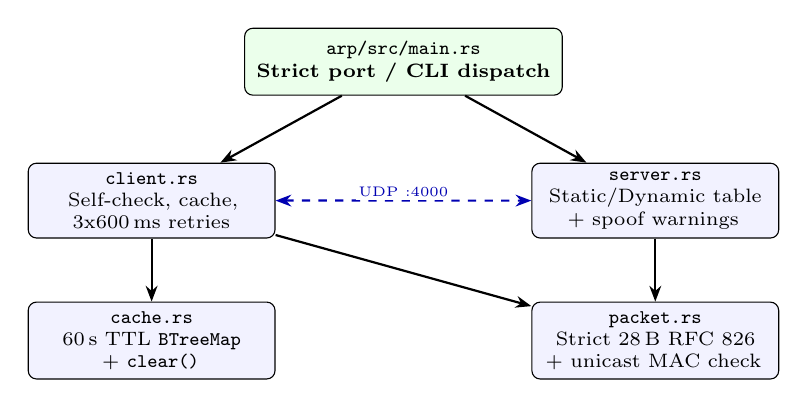
\begin{tikzpicture}[
  box/.style={draw,rounded corners=3pt,fill=blue!5,align=center,font=\scriptsize,minimum height=0.95cm,text width=2.9cm},
  top/.style={draw,rounded corners=3pt,fill=green!8,align=center,font=\scriptsize\bfseries,minimum height=0.85cm,text width=3.8cm},
  arr/.style={-{Stealth[length=2mm]},thick},
  darr/.style={<->,{Stealth[length=2mm]}-{Stealth[length=2mm]},thick,dashed,blue!70!black}
]
  \node[top] (amain) {\texttt{arp/src/main.rs}\\Strict port / CLI dispatch};
  \node[box,below left=0.85cm and -0.4cm of amain] (acli) {\texttt{client.rs}\\Self-check, cache,\\3x600\,ms retries};
  \node[box,below right=0.85cm and -0.4cm of amain] (asrv) {\texttt{server.rs}\\Static/Dynamic table\\+ spoof warnings};
  \node[box,below=0.8cm of acli] (acache) {\texttt{cache.rs}\\60\,s TTL \texttt{BTreeMap}\\+ \texttt{clear()}};
  \node[box,below=0.8cm of asrv] (apkt) {\texttt{packet.rs}\\Strict 28\,B RFC~826\\+ unicast MAC check};

  \draw[arr] (amain) -- (acli);
  \draw[arr] (amain) -- (asrv);
  \draw[arr] (acli) -- (acache);
  \draw[arr] (acli) -- (apkt);
  \draw[arr] (asrv) -- (apkt);
  \draw[darr] (acli) -- node[above,font=\tiny,fill=white,inner sep=1pt]{UDP :4000} (asrv);
\end{tikzpicture}%
}
\end{minipage}\hfill
\begin{minipage}[t]{0.48\textwidth}
\centering
\resizebox{\linewidth}{!}{%
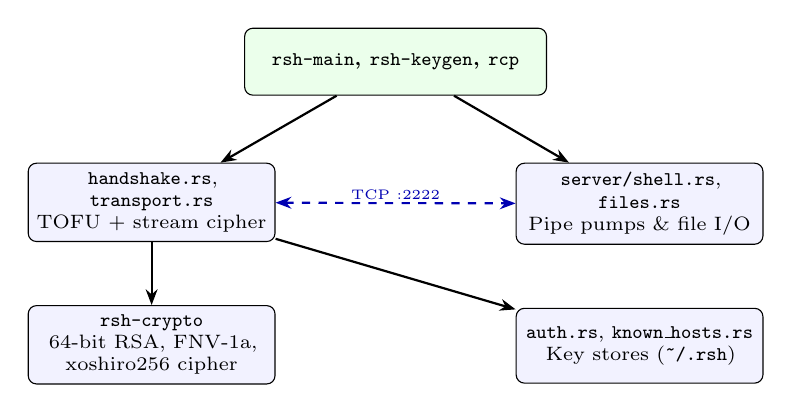
\begin{tikzpicture}[
  box/.style={draw,rounded corners=3pt,fill=blue!5,align=center,font=\scriptsize,minimum height=0.95cm,text width=2.9cm},
  top/.style={draw,rounded corners=3pt,fill=green!8,align=center,font=\scriptsize\bfseries,minimum height=0.85cm,text width=3.6cm},
  arr/.style={-{Stealth[length=2mm]},thick},
  darr/.style={<->,{Stealth[length=2mm]}-{Stealth[length=2mm]},thick,dashed,blue!70!black}
]
  \node[top] (rmain) {\texttt{rsh-main}, \texttt{rsh-keygen}, \texttt{rcp}};
  \node[box,below left=0.85cm and -0.4cm of rmain] (rhnd) {\texttt{handshake.rs}, \texttt{transport.rs}\\TOFU + stream cipher};
  \node[box,below right=0.85cm and -0.4cm of rmain] (rsrv) {\texttt{server/shell.rs}, \texttt{files.rs}\\Pipe pumps \& file I/O};
  \node[box,below=0.8cm of rhnd] (rcry) {\texttt{rsh-crypto}\\64-bit RSA, FNV-1a,\\xoshiro256 cipher};
  \node[box,below=0.8cm of rsrv] (rkey) {\texttt{auth.rs}, \texttt{known\_hosts.rs}\\Key stores (\texttt{\textasciitilde/.rsh})};

  \draw[arr] (rmain) -- (rhnd);
  \draw[arr] (rmain) -- (rsrv);
  \draw[arr] (rhnd) -- (rcry);
  \draw[arr] (rhnd) -- (rkey);
  \draw[darr] (rhnd) -- node[above,font=\tiny,fill=white,inner sep=1pt]{TCP :2222} (rsrv);
\end{tikzpicture}%
}
\end{minipage}
\caption{Modular architecture of the \texttt{arp} (left) and Encrypted Telnet / \texttt{rsh} (right) Cargo projects.}
\label{fig:arch}
\end{figure}

\begin{figure}[H]
\centering
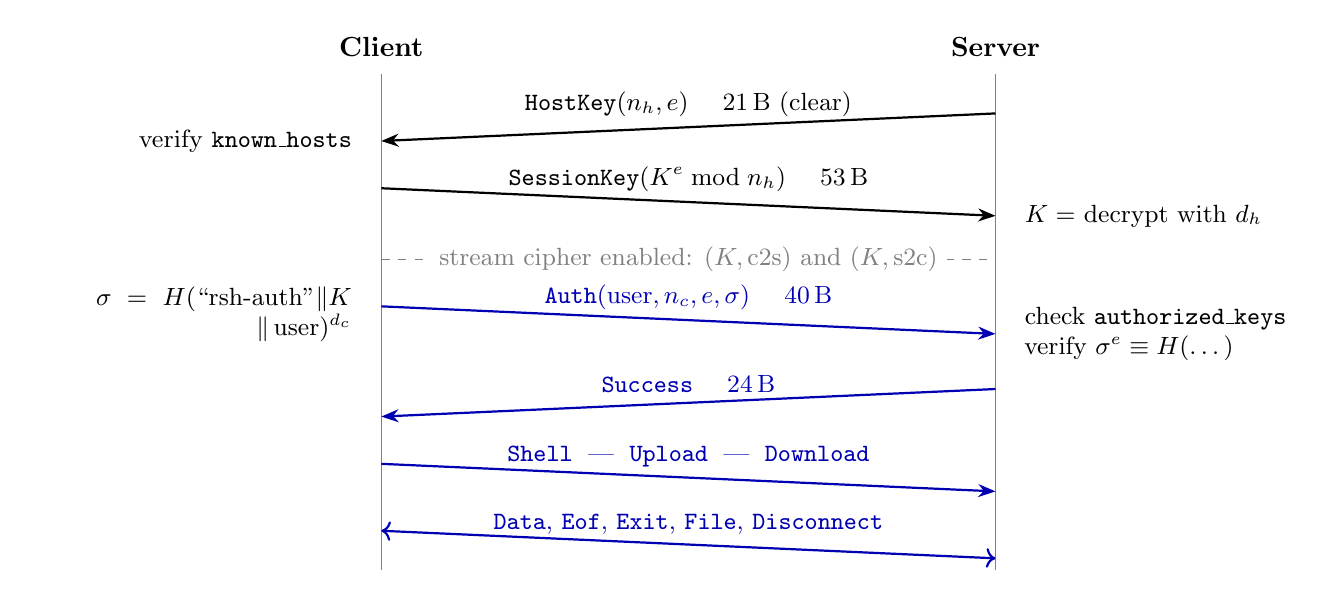
\begin{tikzpicture}[
  font=\small,
  msg/.style={-{Stealth[length=2.2mm]},thick},
  lnote/.style={font=\small,align=right,text width=4.0cm},
  rnote/.style={font=\small,align=left,text width=3.5cm},
]
  \def\L{0} \def\R{7.8}
  \node[font=\bfseries] at (\L,0.35) {Client};
  \node[font=\bfseries] at (\R,0.35) {Server};
  \draw[gray] (\L,0) -- (\L,-6.3);
  \draw[gray] (\R,0) -- (\R,-6.3);

  \draw[msg] (\R,-0.5) -- node[above]{\texttt{HostKey}$(n_h, e)$ \quad 21\,B (clear)} (\L,-0.85);
  \node[lnote,anchor=east] at (\L-0.25,-0.85) {verify \texttt{known\_hosts}};

  \draw[msg] (\L,-1.45) -- node[above]{\texttt{SessionKey}$(K^{e} \bmod n_h)$ \quad 53\,B} (\R,-1.8);
  \node[rnote,anchor=west] at (\R+0.25,-1.8) {$K = $ decrypt with $d_h$};

  \draw[dashed,gray] (\L,-2.35) -- node[fill=white,font=\small]{stream cipher enabled: $(K,\text{c2s})$ and $(K,\text{s2c})$} (\R,-2.35);

  \draw[msg,blue!70!black] (\L,-2.95) -- node[above]{\texttt{Auth}$(\text{user}, n_c, e, \sigma)$ \quad 40\,B} (\R,-3.3);
  \node[lnote,anchor=east] at (\L-0.25,-3.05) {$\sigma = H(\text{``rsh-auth''}\Vert K$\\$\Vert\,\text{user})^{d_c}$};
  \node[rnote,anchor=west] at (\R+0.25,-3.3) {check \texttt{authorized\_keys}\\verify $\sigma^{e} \equiv H(\dots)$};

  \draw[msg,blue!70!black] (\R,-4.0) -- node[above]{\texttt{Success} \quad 24\,B} (\L,-4.35);
  \draw[msg,blue!70!black] (\L,-4.95) -- node[above]{\texttt{Shell} \;|\; \texttt{Upload} \;|\; \texttt{Download}} (\R,-5.3);
  \draw[msg,blue!70!black,<->] (\L,-5.8) -- node[above]{\texttt{Data}, \texttt{Eof}, \texttt{Exit}, \texttt{File}, \texttt{Disconnect}} (\R,-6.15);
\end{tikzpicture}
\caption{The Encrypted Telnet (\texttt{rsh}) handshake. Black arrows are cleartext; blue arrows are encrypted with the stream cipher.}
\label{fig:handshake}
\end{figure}

\subsection{Wire, Input, and Output Formats}

Figure~\ref{fig:wire28} details the 28-byte RFC~826 ARP datagram layout, while Table~\ref{tab:io} summarizes the CLI arguments, interactive inputs, and outputs for all binaries.

\begin{figure}[H]
\centering
\resizebox{\textwidth}{!}{%
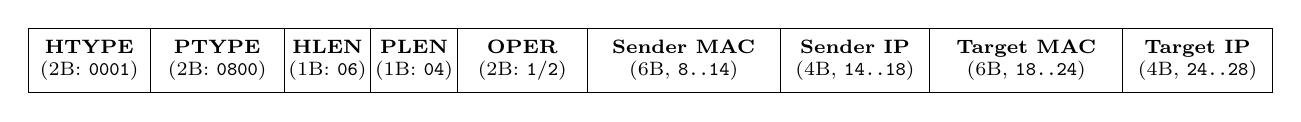
\begin{tikzpicture}[font=\scriptsize]
  \def\h{0.82}
  \draw (0,0)     rectangle (1.55,\h) node[pos=.5,align=center]{\textbf{HTYPE}\\(2B: \texttt{0001})};
  \draw (1.55,0)  rectangle (3.25,\h) node[pos=.5,align=center]{\textbf{PTYPE}\\(2B: \texttt{0800})};
  \draw (3.25,0)  rectangle (4.35,\h) node[pos=.5,align=center]{\textbf{HLEN}\\(1B: \texttt{06})};
  \draw (4.35,0)  rectangle (5.45,\h) node[pos=.5,align=center]{\textbf{PLEN}\\(1B: \texttt{04})};
  \draw (5.45,0)  rectangle (7.10,\h) node[pos=.5,align=center]{\textbf{OPER}\\(2B: \texttt{1}/\texttt{2})};
  \draw (7.10,0)  rectangle (9.55,\h) node[pos=.5,align=center]{\textbf{Sender MAC}\\(6B, \texttt{8..14})};
  \draw (9.55,0)  rectangle (11.45,\h) node[pos=.5,align=center]{\textbf{Sender IP}\\(4B, \texttt{14..18})};
  \draw (11.45,0) rectangle (13.90,\h) node[pos=.5,align=center]{\textbf{Target MAC}\\(6B, \texttt{18..24})};
  \draw (13.90,0) rectangle (15.80,\h) node[pos=.5,align=center]{\textbf{Target IP}\\(4B, \texttt{24..28})};
\end{tikzpicture}%
}
\caption{28-byte RFC~826 ARP packet carried in one UDP datagram (\texttt{arp/src/packet.rs}).}
\label{fig:wire28}
\end{figure}

In \texttt{rsh}, every message is framed over TCP as a 4-byte big-endian length prefix followed by a 1-byte message tag (tags \texttt{1}--\texttt{13}: \texttt{HostKey}, \texttt{SessionKey}, \texttt{Auth}, \texttt{Success}, \texttt{Failure}, \texttt{Shell}, \texttt{Data}, \texttt{Eof}, \texttt{Exit}, \texttt{Upload}, \texttt{Download}, \texttt{File}, \texttt{Disconnect}) and length-prefixed payload fields.

\begin{table}[H]
\centering
\small
\begin{tabularx}{\textwidth}{@{}p{2.3cm} X X@{}}
\toprule
\textbf{Executable} & \textbf{Inputs (CLI, Stdin, Wire)} & \textbf{Outputs (Stdout/Stderr \& Wire)} \\
\midrule
\texttt{arp server} &
CLI: \texttt{arp server [port]} (default \texttt{4000}; invalid port exits via \texttt{usage()}). Wire: exact 28-byte UDP datagrams (\texttt{OP=1}). &
Prints 4 static entries, logs requests, learned dynamic bindings, spoof/MAC-change \texttt{WARNING}s to \texttt{stderr}, and sends 28-byte \texttt{REPLY} (\texttt{OP=2}). \\
\texttt{arp client} &
CLI: \texttt{arp client [my-ip] [server] [port]}. Stdin: IPv4 address, \texttt{cache}, \texttt{flush}, or \texttt{quit}/\texttt{exit}. &
Prints \texttt{Self:}, \texttt{Cache hit:}, \texttt{Sent:} + up to 2 \texttt{Retry} lines, \texttt{Received:}, \texttt{No reply}, sorted cache table with remaining TTL, or \texttt{ARP cache flushed}. \\
\texttt{rsh} / \texttt{rsh-keygen} / \texttt{rcp} &
CLI: \texttt{rsh server [port]}, \texttt{rsh connect <host> [port]}, \texttt{rsh-keygen [-a]}, \texttt{rcp [-P port] <src> <dst>}. Key store in \texttt{\textasciitilde/.rsh}. &
TOFU host key fingerprints, encrypted interactive remote shell (\texttt{sh -i} / \texttt{cmd.exe}), or upload/download progress and exit codes. \\
\bottomrule
\end{tabularx}
\caption{Input and output specifications across the \texttt{arp} and \texttt{rsh} executables.}
\label{tab:io}
\end{table}

% ================================================================ 3
\section{Implementation and Code Guides}

\subsection{ARP Implementation (\texttt{arp/src/})}
\begin{itemize}
  \item \textbf{\texttt{packet.rs} (Strict Wire Codec \& Unicast Check):} \texttt{Mac::from\_ip} derives \texttt{02:00:a:b:c:d} (the locally administered unicast bit set). \texttt{Mac::is\_valid\_unicast} rejects all-zero and multicast/broadcast MACs (\texttt{self.0 != [0; 6] \&\& (self.0[0] \& 1) == 0}). \texttt{ArpPacket::decode} enforces \texttt{b.len() == 28}, \texttt{HTYPE == 1}, \texttt{PTYPE == 0x0800}, \texttt{HLEN == 6}, \texttt{PLEN == 4}, and \texttt{op} $\in \{1, 2\}$.
\end{itemize}

\begin{lstlisting}[caption={Strict packet decoding and unicast MAC check in \texttt{arp/src/packet.rs}.}]
pub fn is_valid_unicast(&self) -> bool {
    self.0 != [0; 6] && (self.0[0] & 1) == 0
}

pub fn decode(b: &[u8]) -> Option<Self> {
    if b.len() != SIZE
        || u16::from_be_bytes([b[0], b[1]]) != HTYPE_ETHERNET
        || u16::from_be_bytes([b[2], b[3]]) != PTYPE_IPV4
        || b[4] != 6 || b[5] != 4
    {
        return None;
    }
    let op = u16::from_be_bytes([b[6], b[7]]);
    if op != REQUEST && op != REPLY { return None; }
    // ... extract sender_mac, sender_ip, target_mac, target_ip
}
\end{lstlisting}

\begin{itemize}
  \item \textbf{\texttt{server.rs} (Static Protection \& Spoof Alert):} Preloaded hosts (\texttt{192.168.1.\{1,10,20,30\}}) are tagged \texttt{EntryKind::Static}. Before learning a sender, the server checks that \texttt{sender\_ip} is non-zero and \texttt{sender\_mac} is a valid unicast address. Static entries refuse overwrites; dynamic entries warn on MAC changes.
\end{itemize}

\begin{lstlisting}[caption={Static-entry protection and MAC-change alerting in \texttt{arp/src/server.rs}.}]
fn learn(table: &mut BTreeMap<Ipv4Addr, Entry>, ip: Ipv4Addr, mac: Mac) {
    match table.get_mut(&ip) {
        None => {
            table.insert(ip, Entry { mac, kind: EntryKind::Dynamic });
            println!("Learned {ip} is at {mac}");
        }
        Some(entry) if entry.mac == mac => {}
        Some(entry) if entry.kind == EntryKind::Static => {
            eprintln!("WARNING: ARP spoof attempt for static IP {ip} (claimed {mac}, keeping {})", entry.mac);
        }
        Some(entry) => {
            eprintln!("WARNING: MAC changed for dynamic IP {ip} ({} -> {mac})", entry.mac);
            entry.mac = mac;
        }
    }
}
\end{lstlisting}

\begin{itemize}
  \item \textbf{\texttt{client.rs} \& \texttt{cache.rs} (Self-Lookup, TTL Cache, \texttt{flush}, and Bounded Retries):} \texttt{Cache} wraps a \texttt{BTreeMap<Ipv4Addr, (Mac, Instant)>} with a 60\,s \texttt{TTL}, lazy \texttt{remove\_expired()}, and \texttt{clear()} for \texttt{flush}. \texttt{Client::resolve} short-circuits self-queries, checks the cache, and otherwise sends up to \texttt{MAX\_RETRIES = 3} requests with a \texttt{600\,ms} per-attempt deadline.
\end{itemize}

\begin{lstlisting}[caption={Self-lookup, cache check, and bounded UDP retry loop in \texttt{arp/src/client.rs}.}]
if target == self.ip {
    println!("Self: {} is at {}", self.ip, self.mac);
    return Ok(());
}
if let Some(mac) = self.cache.get(target) {
    println!("Cache hit: {target} is at {mac}");
    return Ok(());
}
let request = ArpPacket::request(self.mac, self.ip, target);
let encoded = request.encode();
for attempt in 1..=MAX_RETRIES {
    self.socket.send(&encoded)?;
    let deadline = Instant::now() + RETRY_TIMEOUT;
    loop {
        let remaining = deadline.saturating_duration_since(Instant::now());
        if remaining.is_zero() { break; }
        self.socket.set_read_timeout(Some(remaining))?;
        match self.socket.recv(&mut buf) {
            Ok(n) => if let Some(reply) = ArpPacket::decode(&buf[..n]) {
                if reply.op == REPLY && reply.sender_ip == target {
                    self.cache.insert(target, reply.sender_mac);
                    return Ok(());
                }
            },
            Err(e) if matches!(e.kind(), io::ErrorKind::WouldBlock | io::ErrorKind::TimedOut) => break,
            Err(e) => return Err(e),
        }
    }
}
\end{lstlisting}

\subsection{Encrypted Telnet Implementation (\texttt{rsh/src/})}
\begin{itemize}
  \item \textbf{\texttt{rsh-crypto} (\texttt{rsa.rs}, \texttt{prime.rs}, \texttt{cipher.rs}):} Generates two distinct 32-bit primes using 12-base Miller--Rabin (exact for all 64-bit integers), computes $d = e^{-1} \bmod \varphi(n)$, and runs a directional \texttt{xoshiro256}-style stream cipher.
  \item \textbf{\texttt{rsh-main} (\texttt{transport.rs}, \texttt{handshake.rs}, \texttt{shell.rs}):} \texttt{Transport} splits a cloned \texttt{TcpStream} into independent \texttt{Sender} and \texttt{Receiver} halves so shell stdout/stderr pump threads and stdin forwarding run concurrently without deadlocking.
\end{itemize}

\begin{lstlisting}[caption={Key generation (\texttt{rsa.rs}) and directional cipher setup (\texttt{transport.rs}).}]
// rsh-crypto/src/rsa.rs
let p = random_prime(rng, 32);
let q = random_prime(rng, 32);
let phi = (p - 1) * (q - 1);
let Some(d) = inv_mod(EXPONENT, phi) else { continue; };

// rsh-main/src/transport.rs
pub fn encrypt_with(&mut self, key: &[u8], role: Role) {
    let c2s = StreamCipher::new(key, CLIENT_TO_SERVER);
    let s2c = StreamCipher::new(key, SERVER_TO_CLIENT);
    let (outgoing, incoming) = match role {
        Role::Client => (c2s, s2c),
        Role::Server => (s2c, c2s),
    };
    self.sender.cipher = Some(outgoing);
    self.receiver.cipher = Some(incoming);
}
\end{lstlisting}

% ================================================================ 4
\section{Test Cases}

All \textbf{34 automated tests} (\textbf{14} in \texttt{arp/}: 3 unit + 11 black-box integration; \textbf{20} in \texttt{rsh/}: 10 crypto + 3 factoring attack + 7 TCP protocol/handshake) pass after the final edit. Tables~\ref{tab:arptests} and~\ref{tab:rshtests} list every test case, sample stimulus, and verified assertion.

\begin{table}[H]
\centering
\footnotesize
\begin{tabularx}{\textwidth}{@{}>{\ttfamily\scriptsize}l X X l@{}}
\toprule
\normalfont\textbf{Test Case} & \textbf{Sample Input / Stimulus} & \textbf{Checked Behavior} & \textbf{Status} \\
\midrule
mac\_helpers\_work & \texttt{192.168.1.100}, \texttt{Mac::ZERO}, \texttt{ff:..:ff} & Derives \texttt{02:00:c0:a8:01:64}; rejects zero and broadcast MACs & Pass \\
packet\_round\_trip\_and\_strict\_decode & Valid 28B req; 29B buffer; \texttt{op=9} & Valid packet round-trips; 29B trailing byte and \texttt{op=9} return \texttt{None} & Pass \\
insert\_get\_and\_clear & Insert \texttt{192.168.1.10}, call \texttt{clear()} & \texttt{get()} returns \texttt{Some(mac)} before \texttt{clear()} and \texttt{None} after & Pass \\
reply\_has\_rfc826\_layout & 28B req for \texttt{192.168.1.10} & Exact 28-byte RFC~826 reply with \texttt{00:1a:2b:3c:4d:0a} & Pass \\
all\_preloaded\_hosts\_resolve & Requests for \texttt{.1}, \texttt{.10}, \texttt{.20}, \texttt{.30} & All four static hosts return their expected MACs & Pass \\
unknown\_host\_gets\_no\_reply & Request for \texttt{192.168.1.99} & Server drops request; no UDP datagram returned & Pass \\
server\_learns\_the\_sender & Client A (\texttt{10.0.0.5}) asks \texttt{.1}; Client B asks \texttt{10.0.0.5} & Unknown before A's packet; returns A's MAC to B afterward & Pass \\
malformed\_packets\_are\_ignored & Bad \texttt{htype}, \texttt{ptype}, \texttt{hlen}, \texttt{OP=2}, 20B, 29B, empty & All 7 malformed frames ignored; server stays responsive & Pass \\
static\_entry\_cannot\_be\_spoofed & Attacker sends \texttt{SPA=192.168.1.1}, \texttt{SHA=de:ad:be:ef:00:01} & Victim querying \texttt{192.168.1.1} still gets \texttt{00:1a:2b:3c:4d:01} & Pass \\
invalid\_sender\_is\_not\_learned & Requests with \texttt{SPA=0.0.0.0} and \texttt{SHA=00:..:00} & Neither \texttt{0.0.0.0} nor \texttt{10.0.0.99} enters the ARP table & Pass \\
client\_uses\_its\_cache & Stdin: \texttt{.10}, \texttt{.10}, \texttt{cache}, \texttt{quit} & Only 1 UDP \texttt{Sent}; 2nd prints \texttt{Cache hit}; table displays TTL & Pass \\
second\_client\_finds\_the\_first & Client B queries \texttt{.100} and \texttt{not-an-ip} & Resolves A's learned MAC; rejects bad IPv4 cleanly & Pass \\
client\_self\_lookup\_flush\_and\_retries & Stdin: \texttt{.100}, \texttt{.10}, \texttt{flush}, \texttt{.10}, \texttt{.99} & Prints \texttt{Self:}, \texttt{ARP cache flushed}, re-sends \texttt{.10}, 3 tries on \texttt{.99} & Pass \\
udp\_round\_trip\_time & 1000 sequential UDP lookups & Completes all 1000 rounds (39.4\,$\mu$s/req release) & Pass \\
\bottomrule
\end{tabularx}
\caption{Automated unit and black-box integration test cases in \texttt{arp/} (14/14 passing).}
\label{tab:arptests}
\end{table}

\begin{table}[H]
\centering
\footnotesize
\begin{tabularx}{\textwidth}{@{}>{\ttfamily\scriptsize}l X X l@{}}
\toprule
\normalfont\textbf{Test Suite / Cases} & \textbf{Sample Input / Stimulus} & \textbf{Checked Behavior} & \textbf{Status} \\
\midrule
rsh-crypto/tests/crypto.rs (10 tests) & 1000 random moduli; integers <= 200,000; 0--99B RSA blocks; flipped ciphertext bit & Correct modular inverse, Miller--Rabin vs sieve, RSA round-trip, signature verification, stream cipher direction isolation & Pass (10/10) \\
rsh-crypto/tests/attack.rs (3 tests) & 140 moduli (16--64 bits); 10 real \texttt{KeyPair} public keys & Pollard's rho factors 64-bit moduli and recovers real session key + forges signature in 1.32--7.71\,ms & Pass (3/3) \\
rsh-main/tests/protocol.rs (7 tests) & All 13 message tags; truncated/bad-UTF-8 frames; real TCP relay; stranger key; changed host key; replayed login & Framing limits enforced; commands hidden on wire; unauthorized/changed keys rejected; static replay succeeds & Pass (7/7) \\
\bottomrule
\end{tabularx}
\caption{Automated unit, attack, and TCP protocol test suites in \texttt{rsh/} (20/20 passing sequentially).}
\label{tab:rshtests}
\end{table}

% ================================================================ 5
\section{Results}

All benchmarks were executed on macOS (Apple Silicon) over loopback (\texttt{127.0.0.1}) using compiled \texttt{--release} binaries (Rust \texttt{1.99.1}).

\subsection{Captured Wire Exchange and Live Transcripts}
A raw UDP probe from \texttt{192.168.1.100} (\texttt{02:00:c0:a8:01:64}) querying \texttt{192.168.1.20} produced exact 28-byte RFC~826 packets:
\begin{lstlisting}[style=plain]
Request (28B): 00 01 08 00 06 04 00 01 | 02 00 c0 a8 01 64 | c0 a8 01 64 | 00 00 00 00 00 00 | c0 a8 01 14
Reply   (28B): 00 01 08 00 06 04 00 02 | 00 1a 2b 3c 4d 14 | c0 a8 01 14 | 02 00 c0 a8 01 64 | c0 a8 01 64
               <htype><ptyp><hl><pl><op> <--sender MAC---> <-sender IP-> <--target MAC---> <-target IP->
\end{lstlisting}

Live transcript covering Client~1 (\texttt{192.168.1.100}), a spoofing probe for \texttt{192.168.1.1}, Client~2 (\texttt{192.168.1.101}), and invalid sender probes:
\begin{lstlisting}[style=plain]
# Client 1 stdout:
> Self: 192.168.1.100 is at 02:00:c0:a8:01:64
> Sent: ARP Request: who has 192.168.1.10? tell 192.168.1.100 (02:00:c0:a8:01:64)
Received: ARP Reply: 192.168.1.10 is at 00:1a:2b:3c:4d:0a
> Cache hit: 192.168.1.10 is at 00:1a:2b:3c:4d:0a
> ARP cache flushed
> Sent: ARP Request: who has 192.168.1.10? tell 192.168.1.100 (02:00:c0:a8:01:64)
Received: ARP Reply: 192.168.1.10 is at 00:1a:2b:3c:4d:0a
> Sent: ARP Request: who has 192.168.1.99? tell 192.168.1.100 (02:00:c0:a8:01:64)
Retry (2/3): ARP Request: who has 192.168.1.99? tell 192.168.1.100 (02:00:c0:a8:01:64)
Retry (3/3): ARP Request: who has 192.168.1.99? tell 192.168.1.100 (02:00:c0:a8:01:64)
No reply for 192.168.1.99

# Server stderr (spoof attempt, dynamic MAC change, and 0.0.0.0 sender):
WARNING: ARP spoof attempt for static IP 192.168.1.1 (claimed de:ad:be:ef:00:01, keeping 00:1a:2b:3c:4d:01)
WARNING: MAC changed for dynamic IP 192.168.1.100 (02:00:c0:a8:01:64 -> 02:00:aa:bb:cc:dd)
Ignored invalid sender 0.0.0.0 (02:00:00:00:00:01)
\end{lstlisting}

In Encrypted Telnet (\texttt{rsh}), the TCP recording relay (\texttt{handshake\_then\_encrypted\_data}) captured upstream frames \texttt{[53, 40, 29]} bytes (\texttt{SessionKey}, \texttt{Auth}, encrypted 20-byte \texttt{Data} command) and downstream frames \texttt{[21, 24, 24]} bytes (\texttt{HostKey}, \texttt{Success}, encrypted \texttt{Data}): total handshake overhead is \textbf{93\,B upstream} and \textbf{45\,B downstream}, and unlike plaintext Telnet, neither the username nor the shell command appears in cleartext on the wire.

\subsection{Measured Performance Metrics}

Tables~\ref{tab:arpmetrics} and~\ref{tab:rshmetrics} report the measured ARP UDP latencies ($N=200$ requests), \texttt{rsh-crypto} factoring timings, and \texttt{rcp} loopback file-transfer times (median of 5 runs per size; \texttt{rsh} login median across 10 runs was \textbf{10.44\,ms}).

\begin{table}[H]
\centering
\small
\begin{tabular}{@{}l r r r r r@{}}
\toprule
\textbf{ARP Workload} & \textbf{Min} & \textbf{Median} & \textbf{Mean} & \textbf{P95} & \textbf{Max} \\
\midrule
UDP Request/Reply ($N=200$, $\mu$s) & 42.5 & 69.9 & 69.6 & 99.0 & 130.0 \\
Unknown IP ($3\times 600$\,ms retries) & \multicolumn{5}{c}{1810.8\,ms total end-to-end client run (including 6 lookups)} \\
Self-Lookup / Local Cache Hit & \multicolumn{5}{c}{$< 1$\,$\mu$s (in-memory, zero socket I/O)} \\
\bottomrule
\end{tabular}
\caption{Measured ARP resolution latencies over loopback (\texttt{127.0.0.1}).}
\label{tab:arpmetrics}
\end{table}

\begin{table}[H]
\centering
\footnotesize
\begin{tabular}{@{}r r r @{\hspace{14pt}}|@{\hspace{14pt}} r r r@{}}
\toprule
\textbf{Modulus bits} & \textbf{Trial (ms)} & \textbf{Rho (ms)} & \textbf{\texttt{rcp} Size (KB)} & \textbf{Upload (ms)} & \textbf{Download (ms)} \\
\midrule
24 & 0.004 & 0.002 & 1      & 6.51  & 6.35 \\
32 & 0.055 & 0.020 & 16     & 5.99  & 4.98 \\
40 & 1.207 & 0.106 & 256    & 4.49  & 4.40 \\
48 & 9.017 & 0.142 & 1024   & 8.19  & 8.43 \\
56 & --    & 0.911 & 4096   & 14.75 & 13.32 \\
64 & --    & 2.669 & 16384  & 46.08 & 44.30 \\
\bottomrule
\end{tabular}
\caption{Left: mean RSA factoring time (20 moduli/row, \texttt{attack.rs}). Right: median \texttt{rcp} transfer time (5 runs/size).}
\label{tab:rshmetrics}
\end{table}

\subsection{Performance and Protocol Overhead Plots}

Figure~\ref{fig:arpplots} visualizes the measured UDP ARP RTT distribution alongside the resolution path latencies, and Figure~\ref{fig:arpencap} compares wire encapsulation overhead and cumulative lookup savings from the 60\,s TTL cache.

\begin{figure}[H]
\centering
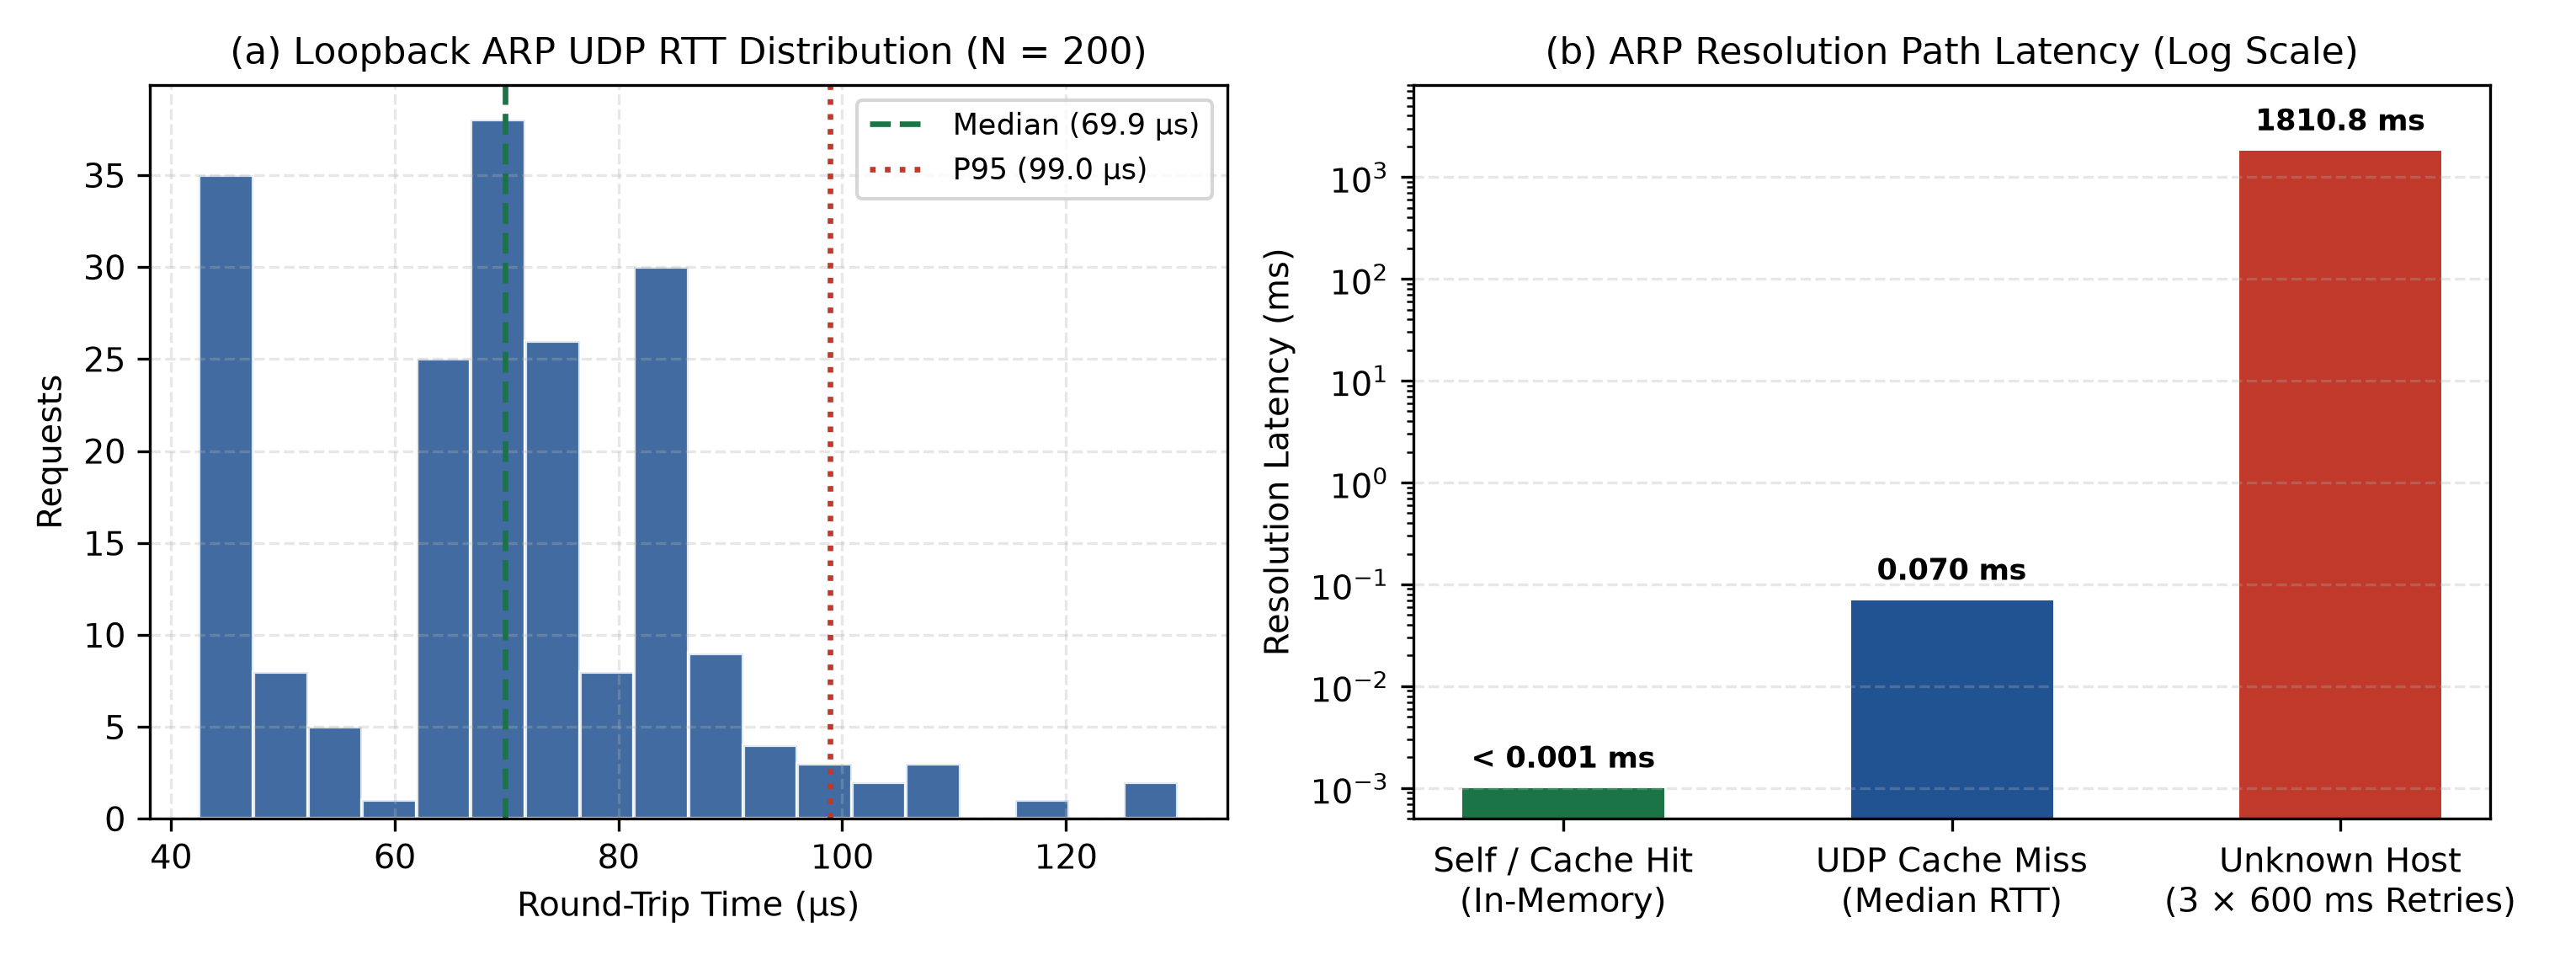
\includegraphics[width=\textwidth]{plots/fig1_arp_rtt.png}
\caption{ARP UDP loopback RTT distribution ($N=200$, median 69.9\,$\mu$s) and resolution path latency comparison.}
\label{fig:arpplots}
\end{figure}

\textbf{Explanation of Figure~\ref{fig:arpplots}:} Loopback UDP lookups complete in 42.5--130.0\,$\mu$s (median 69.9\,$\mu$s, P95 99.0\,$\mu$s). In contrast, self-lookups and cache hits finish in under 1\,$\mu$s in memory, whereas an unknown IP triggers the bounded $3 \times 600\,\text{ms}$ retry sequence (1810.8\,ms measured end-to-end).

\begin{figure}[H]
\centering
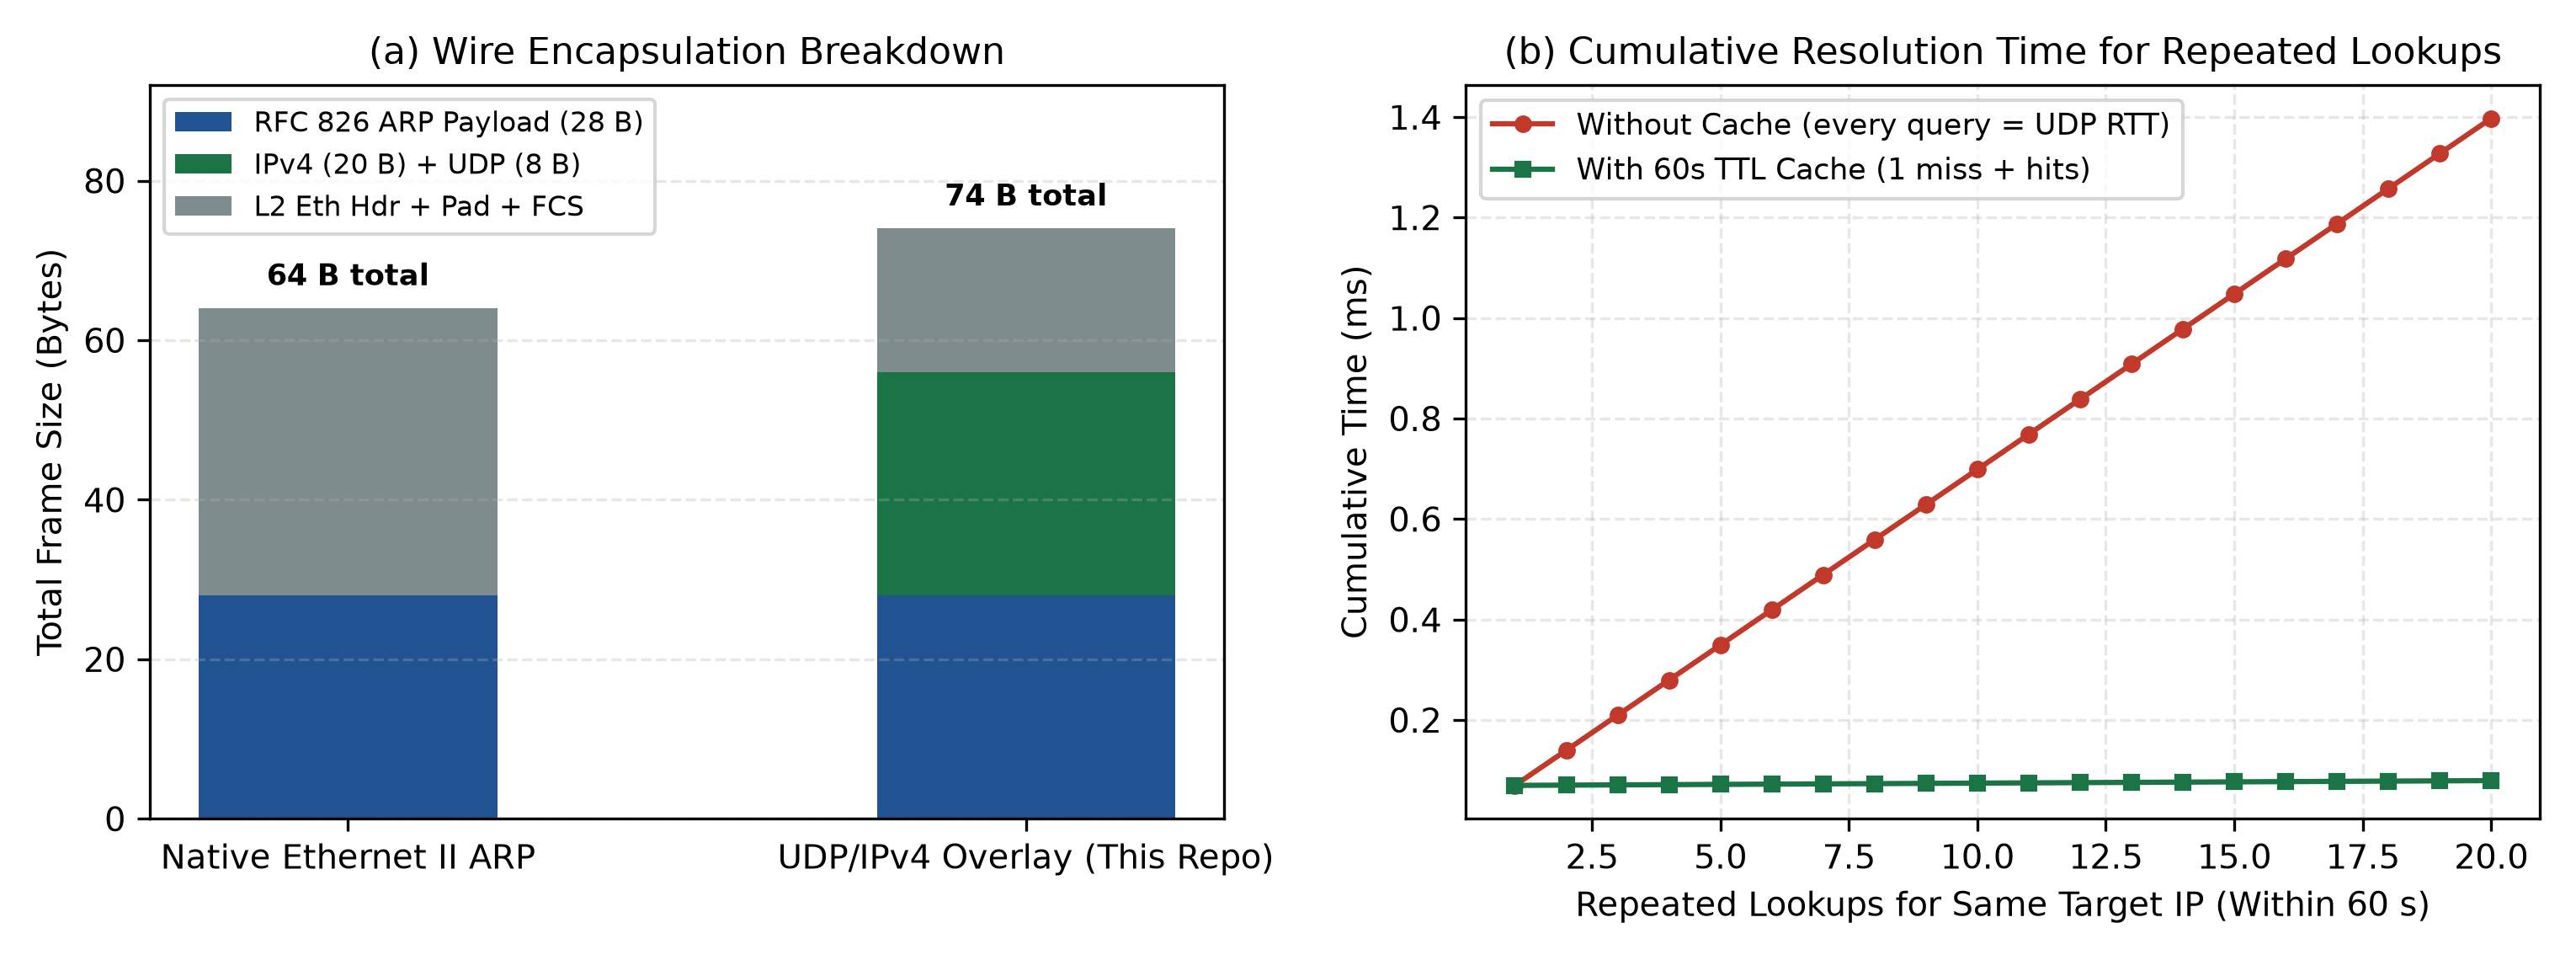
\includegraphics[width=\textwidth]{plots/fig2_arp_encapsulation.png}
\caption{Native Ethernet II ARP (64\,B minimum frame) vs.\ UDP/IPv4 overlay (74\,B with L2), and cumulative lookup time with vs.\ without caching.}
\label{fig:arpencap}
\end{figure}

\textbf{Explanation of Figure~\ref{fig:arpencap}:} Both deployments carry the exact same 28-byte RFC~826 payload. Native Ethernet~II adds 14\,B header + 18\,B zero-padding + 4\,B FCS to meet the 64\,B Ethernet minimum frame size, while our unprivileged UDP/IPv4 overlay adds 20\,B IPv4 + 8\,B UDP headers (56\,B before link framing). Over 20 repeated lookups within 60\,s, caching cuts cumulative wait time from 1.40\,ms (20 UDP round trips) down to $\approx 0.08$\,ms (1 miss + 19 cache hits).

Figures~\ref{fig:rshfactor} and~\ref{fig:rcptransfer} summarize \texttt{rsh-crypto} factoring complexity and \texttt{rcp} loopback scaling.

\begin{figure}[H]
\centering
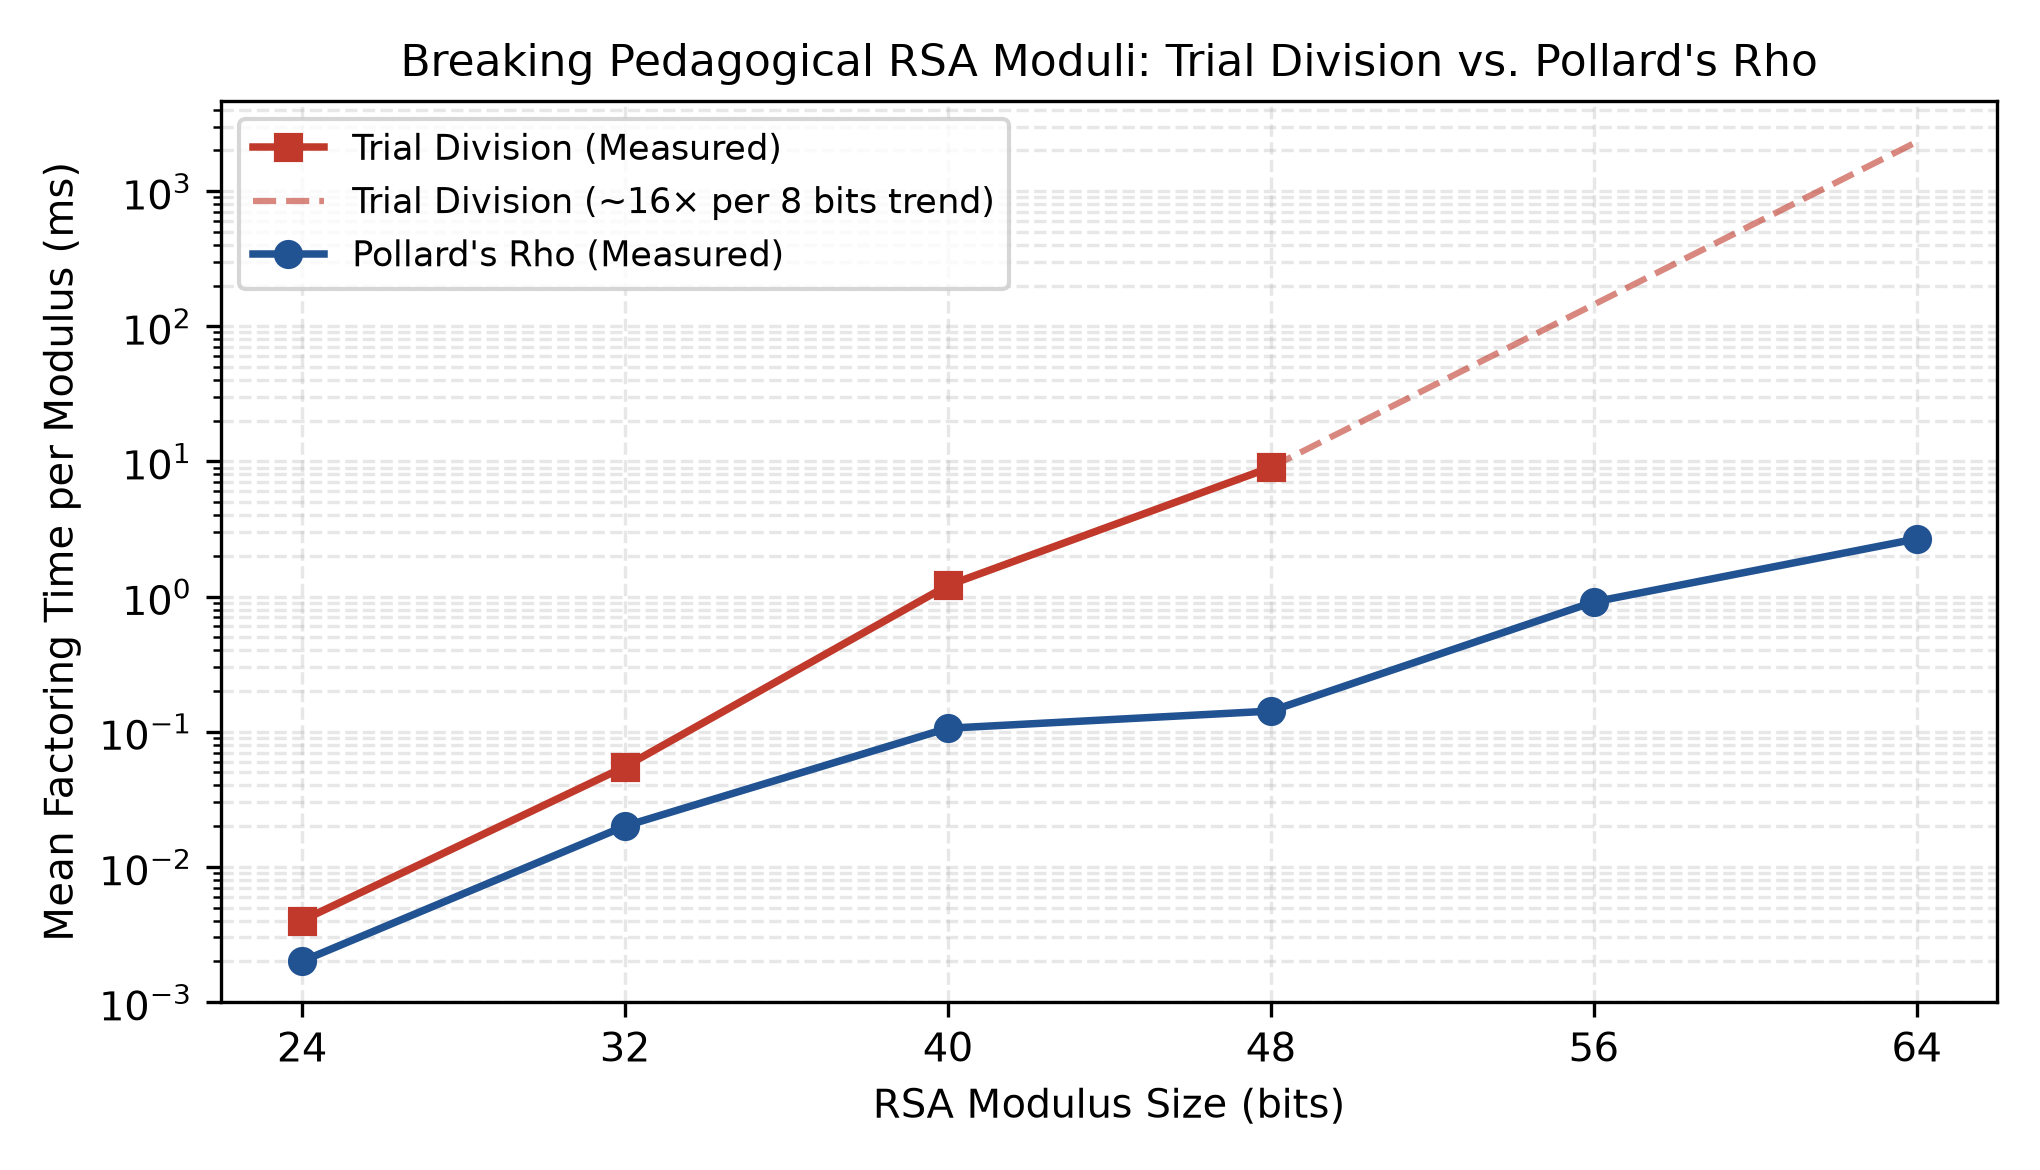
\includegraphics[width=0.76\textwidth]{plots/fig3_rsh_factoring.png}
\caption{Mean RSA factoring time vs.\ modulus size (log scale): Trial Division vs.\ Pollard's Rho.}
\label{fig:rshfactor}
\end{figure}

\begin{figure}[H]
\centering
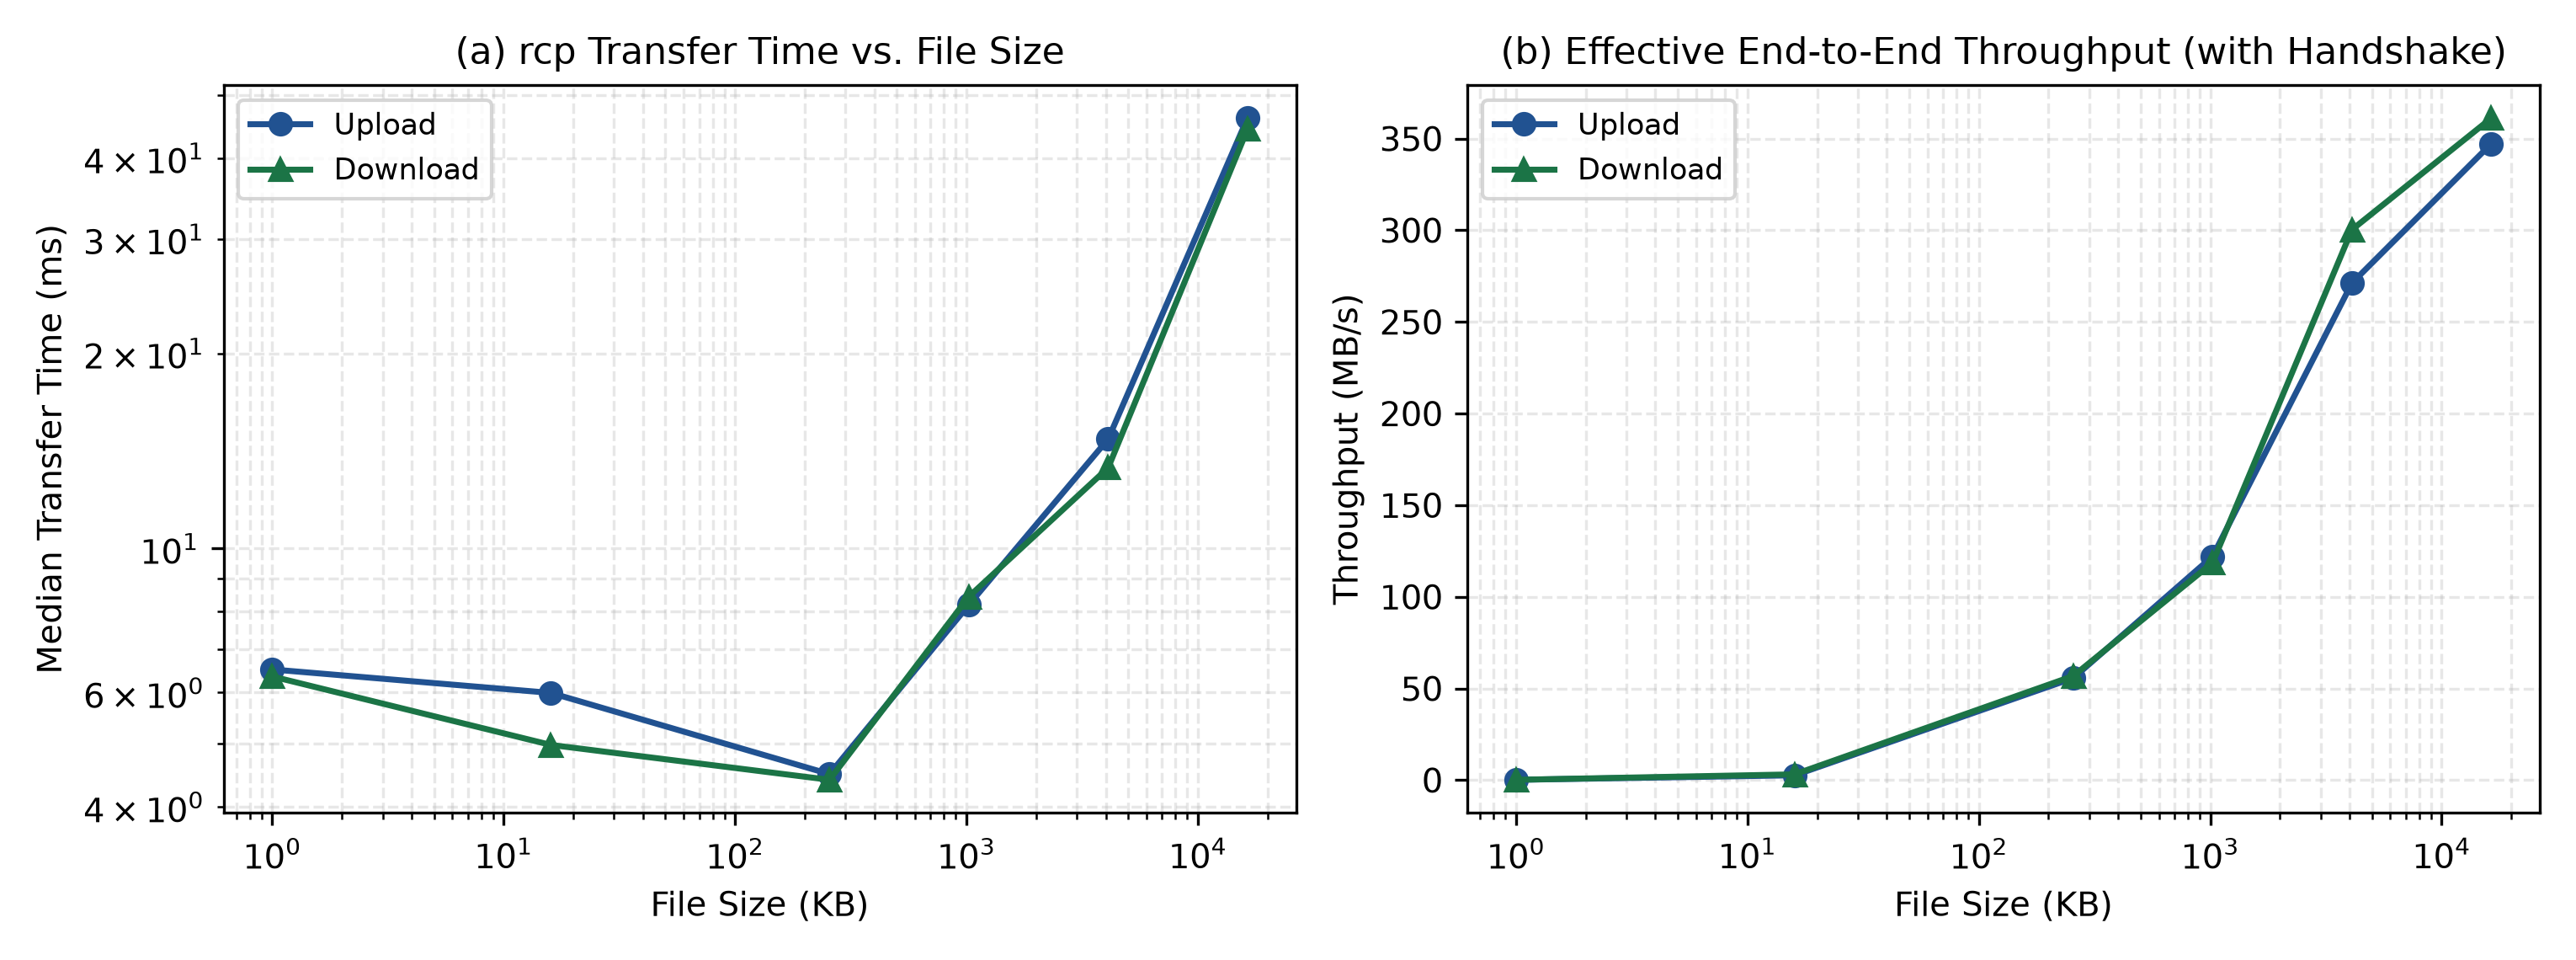
\includegraphics[width=\textwidth]{plots/fig4_rcp_transfer.png}
\caption{\texttt{rcp} median upload/download transfer latency (log-log) and effective end-to-end throughput.}
\label{fig:rcptransfer}
\end{figure}

\textbf{Explanation of Figures~\ref{fig:rshfactor} and~\ref{fig:rcptransfer}:} Trial division grows as $O(n^{1/2})$ ($\approx 16\times$ per 8 bits) and was capped at 48 bits, whereas Pollard's rho grows as $O(n^{1/4})$ ($\approx 4\times$ per 8 bits) and breaks 64-bit moduli in 2.67\,ms on average. In \texttt{rcp}, small files (1--256\,KB) are governed by process start-up and RSA handshake overhead ($\approx 4.4$--$6.5$\,ms), while larger transfers scale smoothly with payload size, reaching $\approx 347$\,MB/s upload and $\approx 361$\,MB/s download at 16\,MB over loopback.

% ================================================================ 6
\section{Analysis}

\subsection{Discussion of Observed Results}
\begin{itemize}
  \item \textbf{ARP Cache, Self-Lookup, and Bounded Retries:} Caching resolved entries for 60\,s and short-circuiting \texttt{self.ip} eliminate $\approx 70$\,$\mu$s UDP lookups on known hosts and avoid the 1.8\,s retry wait on repeated lookups. Splitting the old single 2\,s blocking wait into 3 attempts $\times$ 600\,ms with an explicit per-attempt deadline recovers from isolated UDP datagram drops while bounding worst-case latency.
  \item \textbf{Static Protection vs.\ Dynamic Learning:} Preloaded infrastructure entries (\texttt{192.168.1.1}, \texttt{.10}, \texttt{.20}, \texttt{.30}) cannot be hijacked by spoofed requests, while dynamic peers still auto-register on first contact and trigger clear MAC-change warnings when their hardware address changes.
  \item \textbf{Encrypted Telnet (\texttt{rsh}) Protocol Behavior:} Host-key verification (TOFU), encrypted interactive Telnet-style shell streaming, and file transfers work reliably while hiding usernames and commands from passive sniffers. As expected, 64-bit RSA is strictly educational: Pollard's rho broke all 10 tested host keys in 1.32--7.71\,ms.
\end{itemize}

\subsection{Correctness, Known Limitations, and Edge Cases}
\begin{itemize}
  \item \textbf{Dynamic First-Come Trust in ARP:} While static entries are immutable and MAC changes log warnings, the first host to claim an unseen dynamic IP is trusted without cryptographic authentication (true Dynamic ARP Inspection requires switch-level DHCP snooping bindings).
  \item \textbf{No Server-Side Dynamic Aging or Negative Caching:} Client entries expire after 60\,s, but the server's dynamic table grows indefinitely without a TTL, and querying an unreachable host repeatedly incurs the full 1.8\,s retry delay unless negative caching is added.
  \item \textbf{RSH Cryptographic \& Framing Limits:} Because the client chooses the session key without a server nonce and the stream cipher lacks a MAC, recorded logins can be replayed and ciphertext bits can be flipped (\texttt{flipped\_ciphertext\_bit\_flips\_plaintext\_bit}). Whole-file framing also caps \texttt{rcp} transfers at 64\,MiB.
  \item \textbf{Parallel Test Isolation in \texttt{rsh}:} Protocol integration tests share a fixed temporary \texttt{RSH\_HOME} directory and must be invoked sequentially (\texttt{--test-threads=1}) to avoid \texttt{known\_hosts} races.
\end{itemize}

\subsection{Possible Improvements}
\begin{itemize}
  \item \textbf{ARP:} Add server-side TTL aging for dynamic entries, short-lived client negative caching (e.g., 5\,s) for unreachable IPs, and optional Gratuitous ARP / Duplicate Address Detection (RFC~5227) announcements on startup.
  \item \textbf{RSH:} Move to $\ge$2048-bit RSA (or ECDH) with a server challenge nonce, add per-frame AEAD / HMAC-SHA256 authentication with sequence numbers, stream \texttt{rcp} files in chunks to lift the 64\,MiB limit, and combine length-prefix + payload writes (or set \texttt{TCP\_NODELAY}).
\end{itemize}

\end{document}
